% !TEX encoding = UTF-8 Unicode
% REMEMBER TO SET LANGUAGE!
\documentclass[a4paper,10pt,norsk]{article}
\usepackage[utf8]{inputenc}
\usepackage[norsk]{babel}
% Standard stuff
\usepackage{amsmath,graphicx,varioref,verbatim,amsfonts,geometry}
% colors in text
\usepackage[usenames,dvipsnames,svgnames,table]{xcolor}
% Hyper refs
\usepackage[colorlinks]{hyperref}

% Document formatting
\setlength{\parindent}{0mm}
\setlength{\parskip}{1.5mm}

%Color scheme for listings
\usepackage{textcomp}
\definecolor{listinggray}{gray}{0.9}
\definecolor{lbcolor}{rgb}{0.9,0.9,0.9}

%Listings configuration
\usepackage{listings}
%Hvis du bruker noe annet enn python, endre det her for å få riktig highlighting.
\lstset{
	backgroundcolor=\color{lbcolor},
	tabsize=4,
	rulecolor=,
	language=python,
        basicstyle=\scriptsize,
        upquote=true,
        aboveskip={1.5\baselineskip},
        columns=fixed,
	numbers=left,
        showstringspaces=false,
        extendedchars=true,
        breaklines=true,
        prebreak = \raisebox{0ex}[0ex][0ex]{\ensuremath{\hookleftarrow}},
        frame=single,
        showtabs=false,
        showspaces=false,
        showstringspaces=false,
        identifierstyle=\ttfamily,
        keywordstyle=\color[rgb]{0,0,1},
        commentstyle=\color[rgb]{0.133,0.545,0.133},
        stringstyle=\color[rgb]{0.627,0.126,0.941}
        }
        
\newcounter{subproject}
\renewcommand{\thesubproject}{\alph{subproject}}
\newenvironment{subproj}{
\begin{description}
\item[\refstepcounter{subproject}(\thesubproject)]
}{\end{description}}

%Lettering instead of numbering in different layers
%\renewcommand{\labelenumi}{\alph{enumi}}
\renewcommand{\thesubsection}{\alph{subsection}}

%opening
\title{FYS-MEK 1110 - Oblig 2}
\author{Joakim Flatby}

\begin{document}

\maketitle
\section{}


%Oppg a
\subsection{)}

\begin{figure}[h!]
        \centering 
        \includegraphics[scale=1.0]{chart2.png} 
        \caption{Free Body Diagram of a ball on a pendulum(Drawn with draw.io)}
\end{figure}

%Oppg b
\subsection{)}
Show that the net force can be written as:
\[\sum{\vec{F} = -mgj - k(r-L_{0}) \frac{\vec{r}}{r}}\]

Modeling the rope as a spring, $\vec{T}$ can be found using $F = -kx$:

\[\vec{T} = -k(r-r_{0})\frac{\vec{r}}{r}\]

and $\vec{G}$ can be found by using $F = mgh$. In our case the height(length of the Y-position-vector) is j

\[\vec{G} = -mgj\]

\[\sum{\vec{F}} = \vec{T} + \vec{G}\]
\[\sum{\vec{F} = -k(r-L_{0}) \frac{\vec{r}}{r}} -mgj\]
which equals:
\[\sum{\vec{F} = -mgj - k(r-L_{0}) \frac{\vec{r}}{r}}\]

%Oppg c
\subsection{)}

\[\vec{r}(t) = x(t)i + y(t)j\]
Rewriting the external force on component form:
Replacing $\vec{r}$ with x(t) in the x-formula, and same with y(t), replacing r with $| \vec{r} | = \sqrt{x(t)^{2} + y(t)^{2}}$ and removing gravity from the x-formula

\[\vec{F}_{x}(t) = -k\Big(\sqrt{x(t)^{2} + y(t)^{2}} - L_{0} \Big)\frac{x(t)}{\sqrt{x(t)^{2} + y(t)^{2}}}\]

\[\vec{F}_{y}(t) = -mg - k\Big(\sqrt{x(t)^{2} + y(t)^{2}} - L_{0} \Big)\frac{y(t)}{\sqrt{x(t)^{2} + y(t)^{2}}}\]

%oppg d
\subsection{)}
The angle $\theta$ does not give a sufficient description of the position in our case because we are treating the rope as a spring, and therefore giving allowing it to change length. So to find the position of the ball we would need the length of the rope at that time, as well as the angle.

% oppg e
\subsection{)}
If the ball is at rest with $\theta = 0$, the x-position $x(t) = 0$ because the ball is straight under (0, 0), where the rope is attached. If we put this into the component formulas from task C, we get
\[\vec{F}_{x}(t) = -k\Big(\sqrt{0 + y(t)^{2}} - L_{0} \Big)\frac{0}{\sqrt{0 + y(t)^{2}}} = 0\]
\[\vec{F}_{x}(t) = 0\]

and because the ball is at rest with no acceleration, we know that the tension force $|\vec{T}|$ is equal to the gravity force $|\vec{G}|$: 

\[- k\Big(\sqrt{x(t) + y(t)^{2}} - L_{x(t)} \Big)\frac{y(t)}{\sqrt{x(t)^{2}+ y(t)^{2}}} = mg\]
therefore:

\[k\Big(\sqrt{0 + y(t)^{2}} - L_{0} \Big)\frac{y(t)}{\sqrt{0 + y(t)^{2}}} = mg\]
\[- k\Big(y(t) - L_{0} \Big)\frac{y(t)}{\pm y(t)} = mg\]
\[- k\Big(y(t) - L_{0}\frac{y(t)}{\pm y(t)}\Big) = mg\]
\[- k\Big(y(t) \pm L_{0}\Big) = mg\]

\[- k\Big(y(t) \pm L_{0} \Big) = mg\]
\[y(t) \pm L_{0} = -\frac{mg}{k}\]
\[y(t) = \pm L_{0} -\frac{mg}{k}\]

So the position of the ball is:
\[\vec{r} = \Big[0, \pm L_{0} - \frac{mg}{k}\Big]\]

if you increase the value k, the length (or y-position) would be smaller because the rope would stretch less from the natural weight of the ball.

%oppg f
\subsection{)}

Vector form:
\[\vec{a} = \frac{\sum{F}}{m} = -gj - \frac{k(r-L_{0})}{m}\frac{\vec{r}}{r}\]
\[ = -9.81j - 2000(r-1)\frac{\vec{r}}{r}\]

Component form:
\[a_{x} = -200\Big(\sqrt{x^{2} + y^{2}} - 1 \Big) \frac{x}{0.1\sqrt{x^{2} + y^{2}}}\]
\[a_{y} = -9.81 - 200\Big(\sqrt{x^{2} + y^{2}} - 1 \Big) \frac{y}{0.1\sqrt{x^{2} + y^{2}}}\]

%oppg g
\subsection{)}
\[\vec{v} = v_{0} + \int_{0}^{t}a \  dt\]
\[v_{0} = 0\]
\[\vec{v} = at\]
\[\vec{r} = \int_{0}^{t} at \ dt\]
\[\vec{r} = \frac{1}{2} at^{2} + C\]
\[C = r_{0}\]
\[\vec{r} = r_{0} + \frac{1}{2} at^{2}\]
\[r_{0} = 1\]
 
 %oppg h
 \subsection{)}
 \[\vec{v}(t + \Delta t) = \vec{v}(t) + \Delta t * \vec{a}\big(x(t), v(t), t\big)\]
 \[\vec{r}(t + \Delta t) = \vec{r}(t) + \Delta t * \vec{v}\big(t + \Delta t\big)\]
 
 \[\vec{a}(t + \Delta t) = -9.81 - 2000\big(\vec{r}(t + \Delta t) - 1\big)\frac{\vec{r}(t + \Delta t)}{r(t + \Delta t}\]
 
 %oppg i
 \subsection{)}
 \lstinputlisting{oppg_i.py}
 
 %oppg j
 \subsection{)}
 
 \begin{figure}[h!]
        \centering 
        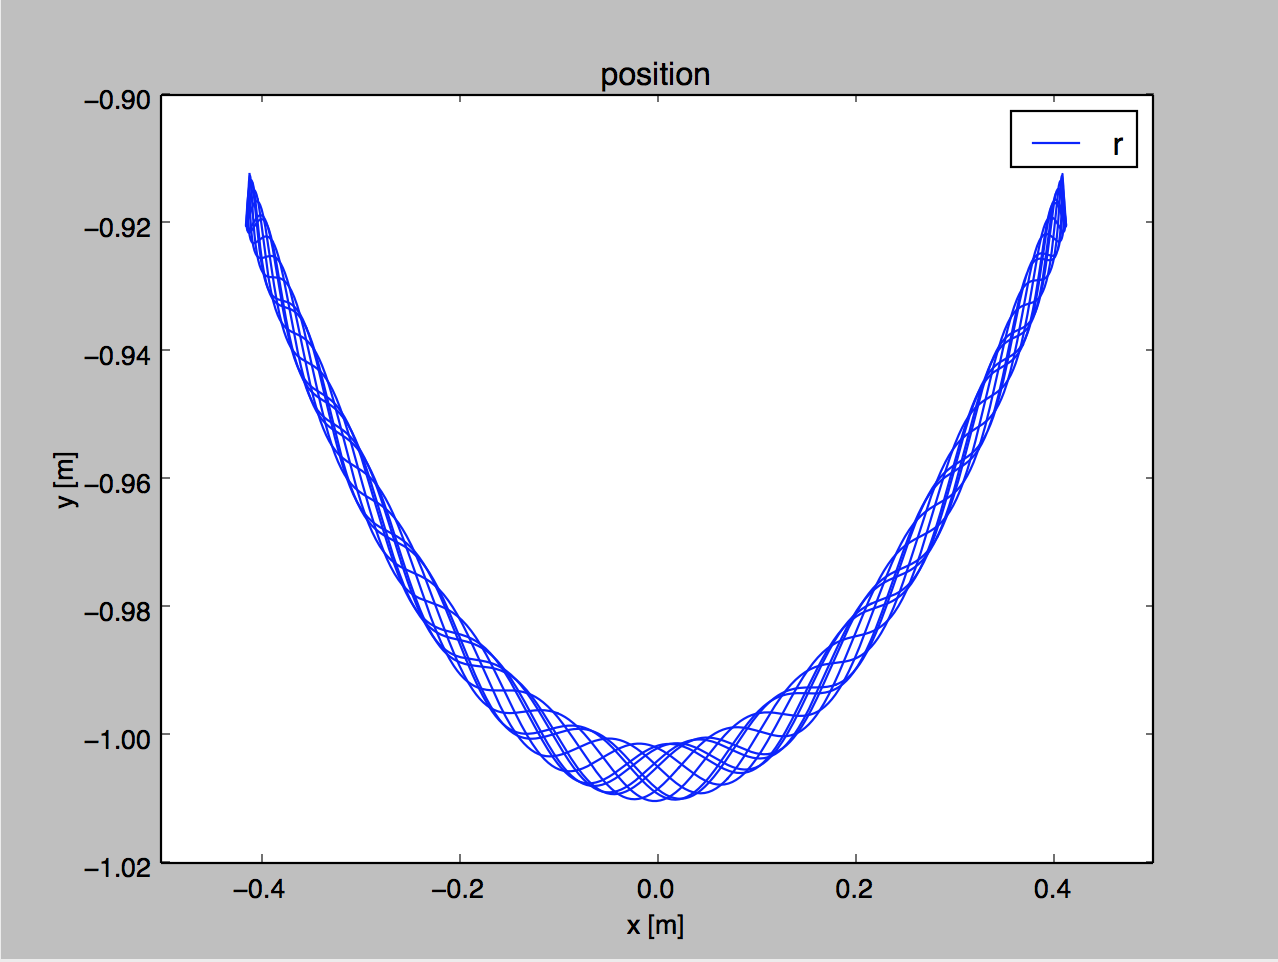
\includegraphics[scale=0.4]{oppg_j.png} 
        \caption{PyPlot with $\Delta t$ = 0.001}
\end{figure}
 
 What I see is that the ball is following a parabolic path, with some variation because of the fact that we are treating the rope as a spring.
 
 %oppg k
 \subsection{)}
 
 \begin{figure}[h!]
        \centering 
        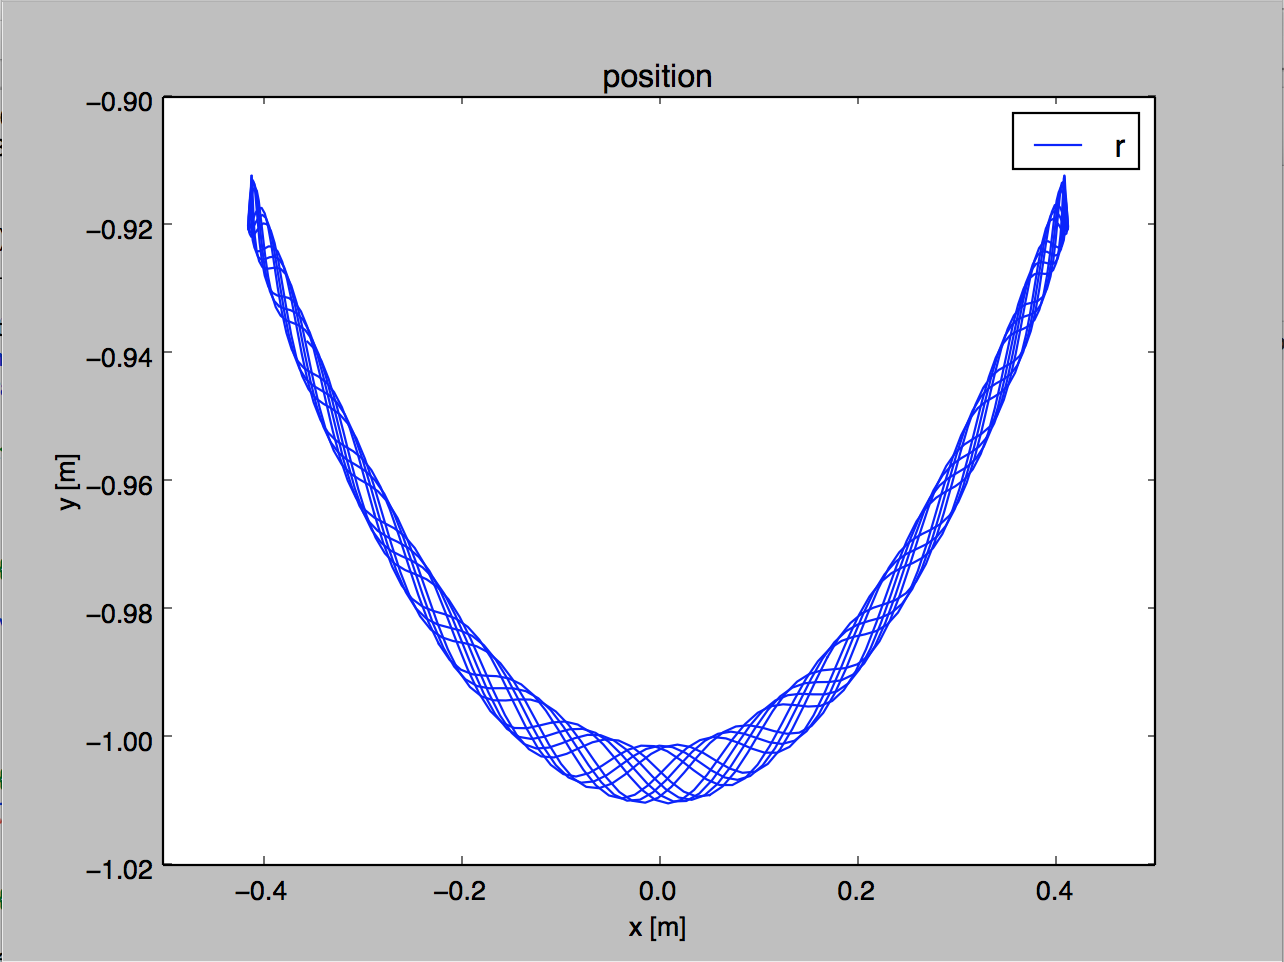
\includegraphics[scale=0.4]{oppg_k_0,01.png} 
        \caption{PyPlot with $\Delta t$ = 0.01}
\end{figure}

\begin{figure}[h!]
        \centering 
        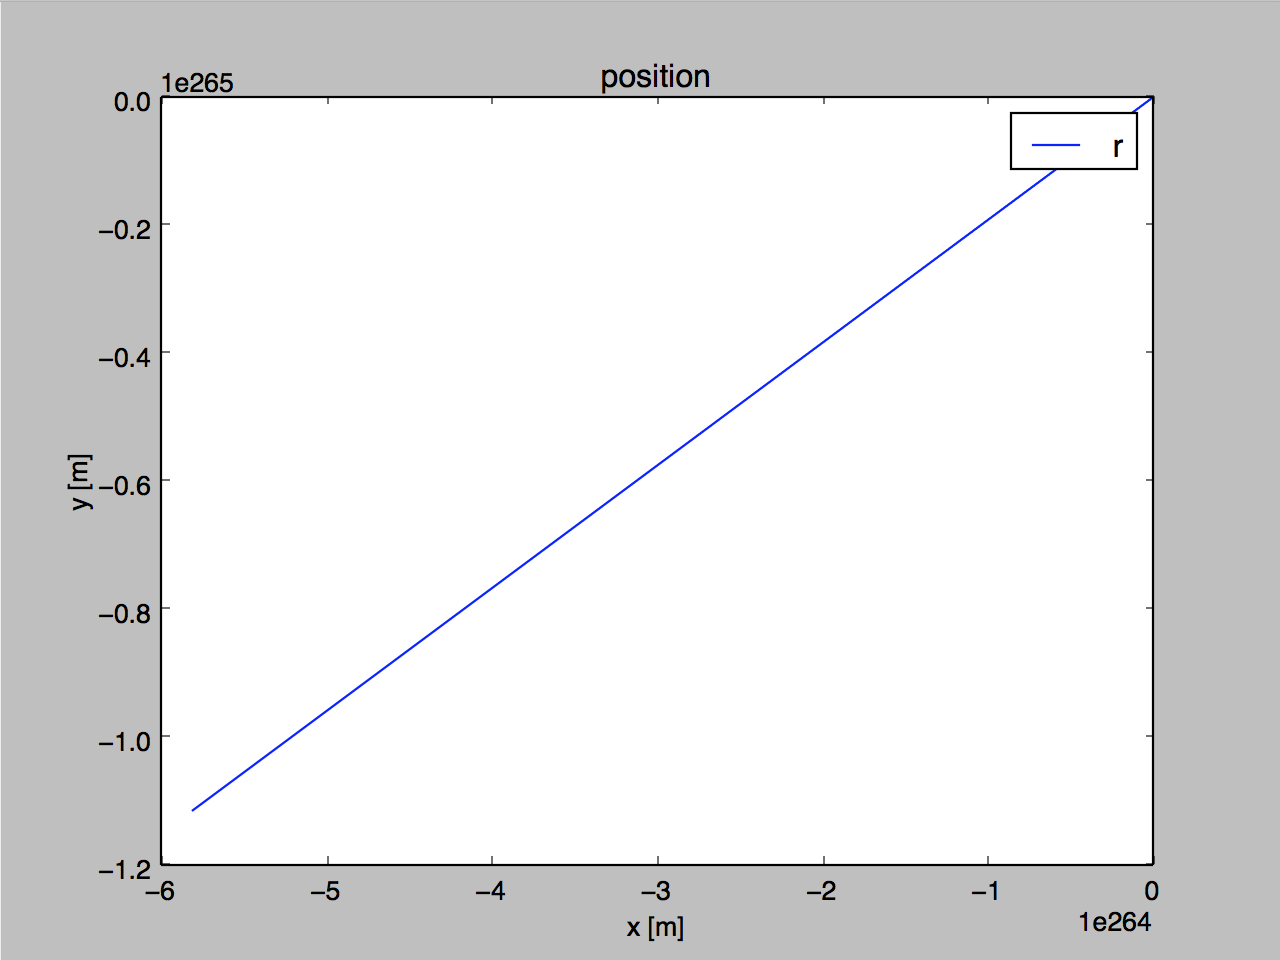
\includegraphics[scale=0.4]{oppg_k_0,1.png} 
        \caption{PyPlot with $\Delta t$ = 0.1}
\end{figure}
 
When $\Delta t$ increases, the plot is getting less dense because of less lines following roughly the same path with a little wiggle-room because of the ropes ability to stretch..

Setting $\Delta t$ to 0.1 gives an error and only returns a straight line with my code..
 
 %oppg l
 \subsection{)}
 \begin{figure}[h!]
        \centering 
        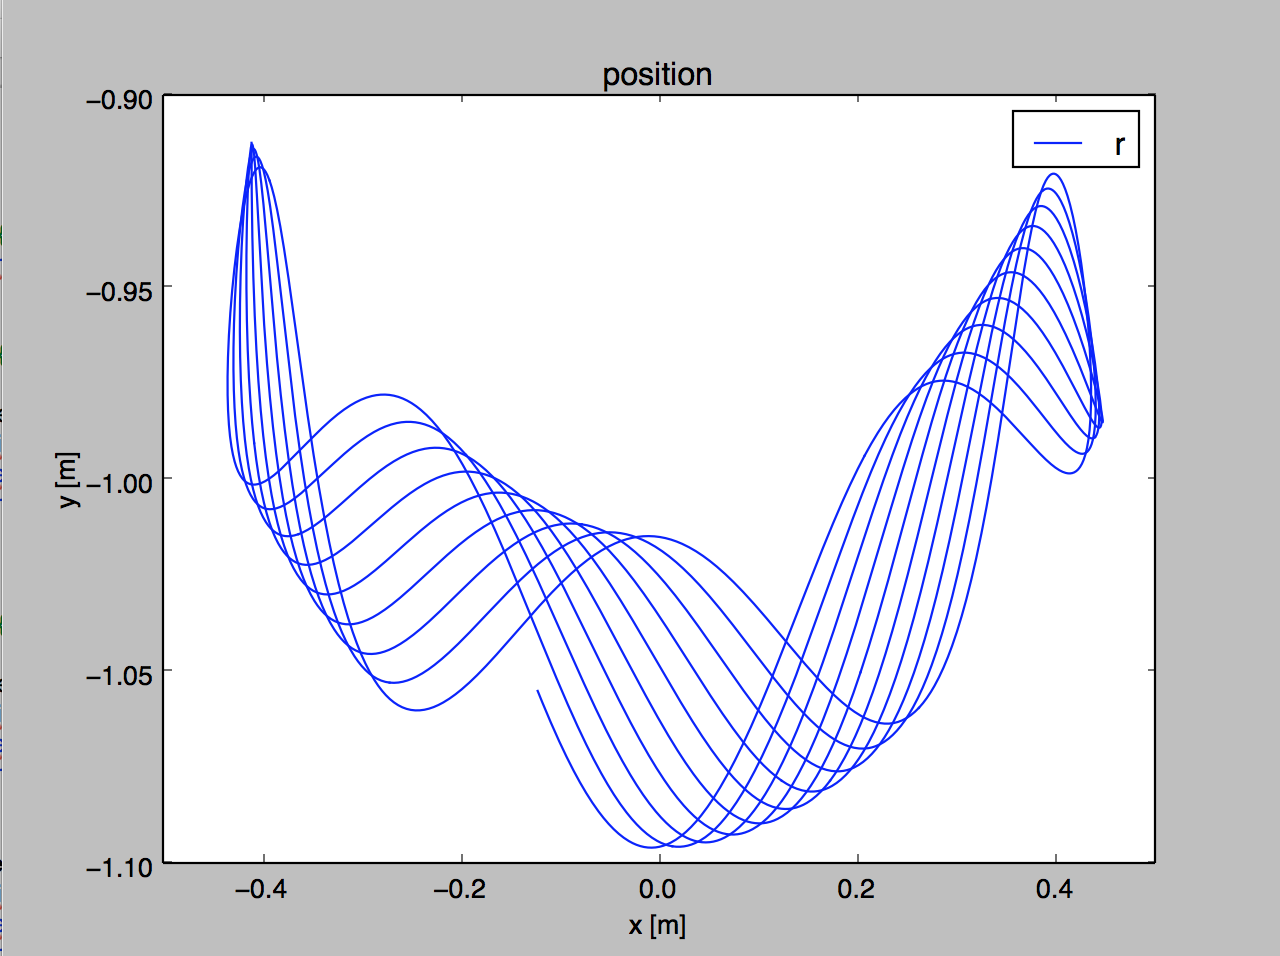
\includegraphics[scale=0.4]{oppg_l_20.png} 
        \caption{PyPlot with $k = 20$}
\end{figure}
\begin{figure}[h!]
        \centering 
        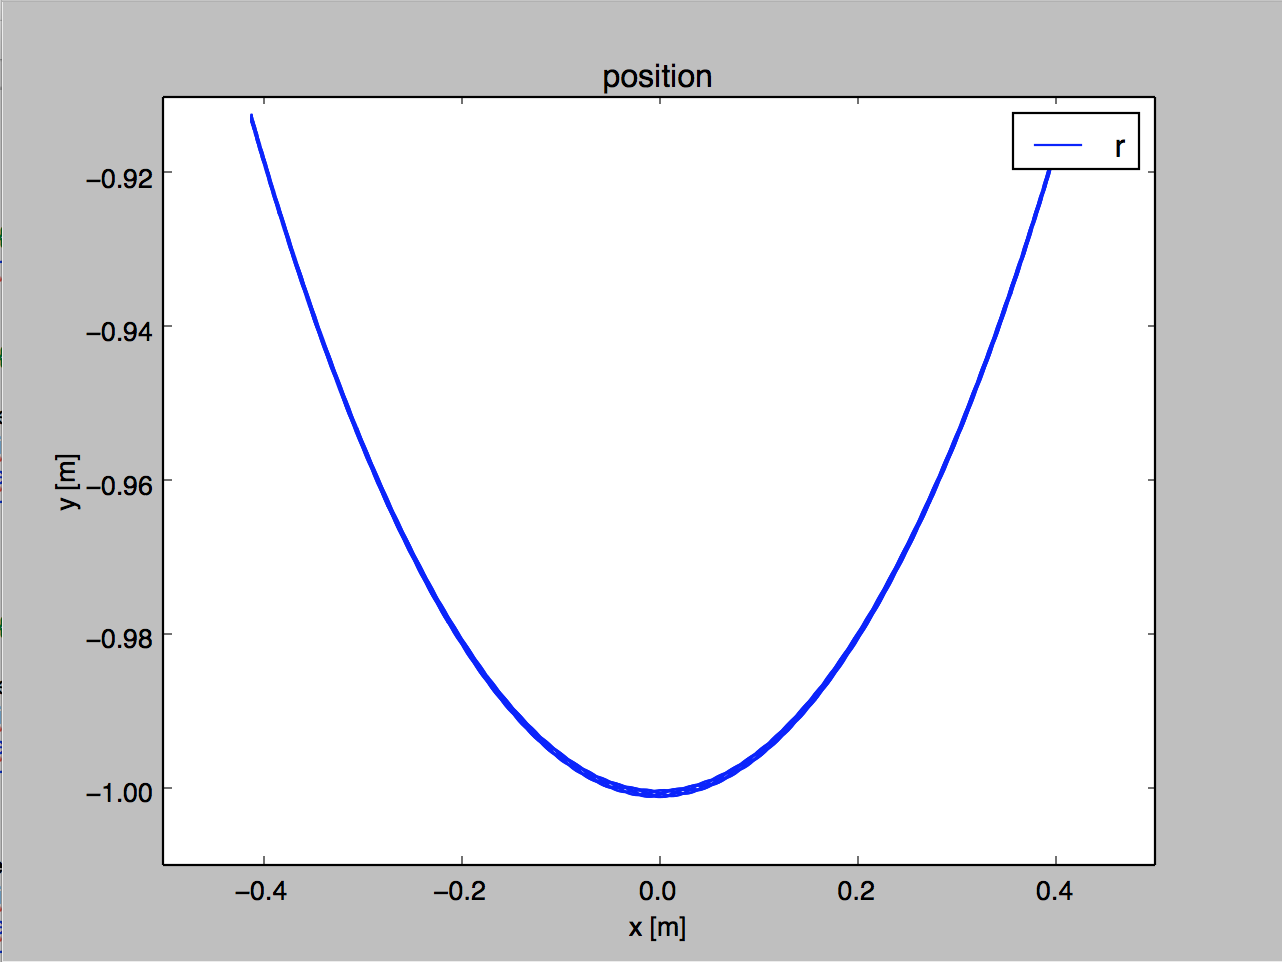
\includegraphics[scale=0.4]{oppg_l_2000.png} 
        \caption{PyPlot with $k = 2000$}
\end{figure}
 When k is lowered, the rope is allowed to stretch more, and the position-plot will vary more (resulting in a ``thicker`` plot bacause it moves further away from the path it would follow with a stiff rope.)
 When k is increased the lines almost go together to a point where it looks like the plot is just one line following a parabolic path.
 
 %oppg m
 \subsection{)}
 I see now that I changed the orininal code for task i, but I guess that doesnt matter. The only change apart from the different inital values, is that instead of calculating the rope tension S normally, I send it through a function that returns 0 if the rope length is shorter than the initial rope length.
 
 The result of plotting with these initial values for me is circular motion.
 I guess this is because the initial velocity is so high that the ball would take several rounds before gravity is enough to push it back down on the same side it came up.
 
 If I lower the rope tension K, the ball follows a much less circular route(still round though), and it comes to rest faster because of losing more energy.
 \begin{figure}[h!]
        \centering 
        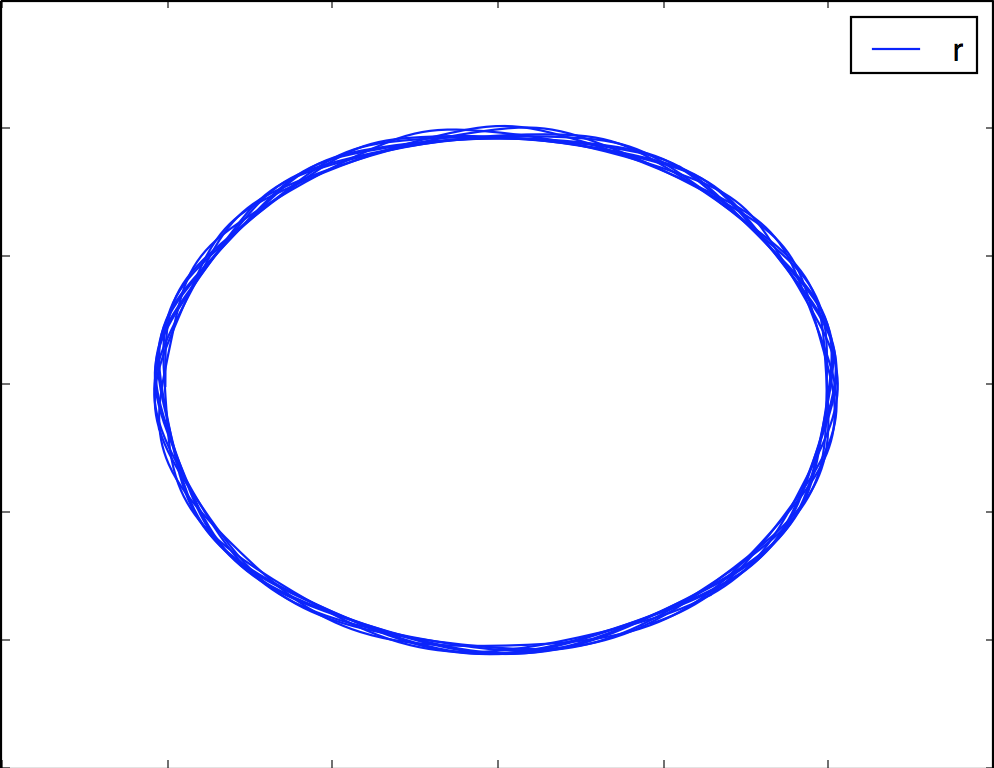
\includegraphics[scale=0.5]{oppg_m.png}
\end{figure}
 
 
\end{document}